\section{PID-Regler \formelbuch{147}}

	\subsection{P-Regler - Stationärer Zustand \formelbuch{155}}
		Beim einfachsten linearen Regler, dem P-Typ, besteht ein proportionaler
		Zusammenhang zwischen Fehler $e$ und Stellgrösse $u$.\\
		Der P-Regler reagiert schnell, kann aber den Sprungfehler nicht vollständig
		eliminieren. Er hat einen stationären Fehler.
		
	
	\subsection{I-Regler \formelbuch{160}}
		Der reine I-Regler ist allgemein ungünstig, weil er relativ langsam arbeitet
		und die Stabilität schwächt. Ist aber die Regelstrecke nur erster Ordnung
		erziehlt man gute Ergebnisse mit dem I-Regler.\\
		Der I-Regler neigt zum Schwingen.\\
		Bei sprungförmigen Signalen, d.h. für Festwertregelungen hat der I-Regler
		keinen Fehler!
		
	
	\subsection{$PT_2$-Glied \formelbuch{163}}
		\begin{minipage}{5cm}
        \fbox{$T_\omega = 2T_m=\frac{2\pi}{\omega_n \sqrt{1-\zeta
        ^2}}=\frac{2\pi}{\omega}$}\\
        \fbox{$\omega = \frac{2\pi}{T_\omega}=2\pi f$}
        \end{minipage}
		\begin{minipage}{13cm}
        $T_\omega$: Schwingungsdauer\\
        $\omega_n$: Kennkreisfrequenz\\
        $\zeta$: \hspace{1.1mm} Dämpfungskonstante\\
        \end{minipage}\\
		\glqq Optimale Dämpfung\grqq\ bei $\Psi=45$ und $\zeta=\frac{1}{\sqrt{2}}$.
		Dabei erreicht die Regelgrösse $y$ nach $4.3\%$ Überschwingen rasch den
		Endwert.\\
		\begin{minipage}{7cm}
		$T^2\ddot{y}+2\zeta T \dot{y}+ y=Ku$\\
		$\ddot{y}+2\zeta\omega_n\dot{y}+\omega_n^2=\omega_n^2 Ku$
		\end{minipage}
		\begin{minipage}{11cm}
        $\ddot{y}+a_1\dot{y}+a_0 y=\ldots$\\
        $a_1=2\zeta\omega_n$\\
        $a_0=\omega_n^2$
        \end{minipage}
	
	\subsection{PI-Regler \formelbuch{174}}
		\begin{minipage}{15cm}
        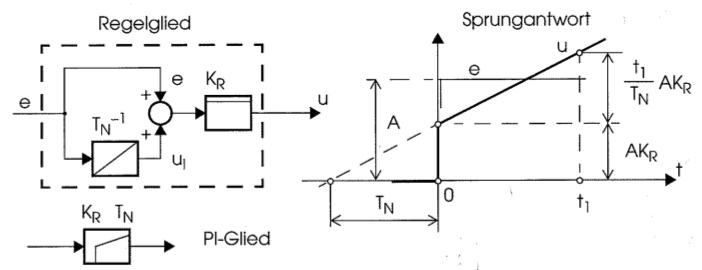
\includegraphics[angle={0},width=10cm]{./bilder/PI_Regler.jpg}
        \end{minipage}\\ \\
		\begin{minipage}{15cm}
        \fbox{$G(j\omega)=K_R \frac{1+j\omega T_N}{j\omega T_N}$}\qquad
        \fbox{$arg(G(j\omega))=\arctan(\omega T_N)-\frac{\pi}{2}$}
        \end{minipage}
		
	
	\subsection{D-Glied \formelbuch{179}}
		Der Differenzierer erzeugt eis Korrektursignal im voraus.\\
		Nachteilig ist, wenn die Regelgrösse verrauscht ist, dann werden die
		hochfrequenten Störsignale durch die Ableitung verstärkt.\\
		Ein LTI-System, welches ohne D-Glied darstellbar ist, gegebenenfalls durch
		Umformung des Blockdiagramms, heisst realisierbar.
	
	
	\subsection{PID-Regler \formelbuch{183} \formelbuch{383}}
	\fbox{$G(s) = K_R(1 + \frac{1}{j \omega T_N} + j \omega T_V )$}
	
	\subsection{PD-Regler \formelbuch{187} \formelbuch{383}}
	\fbox{$u=K_R at+K_R T_V a$} \qquad
	Das PD-Glied entspricht dem inversen PT$_1$-Glied.
	
	\subsection{Empirische Einstellregeln \formelbuch{188}}
		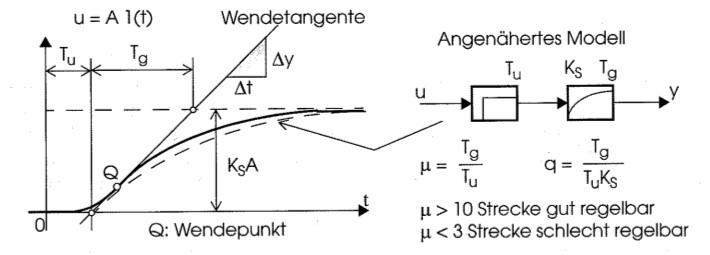
\includegraphics[width=13cm]{./bilder/Empirisch_Regeln.jpg}
		\begin{minipage}[b]{5cm}
        UTF des angenäherten Modells:\\ \\
		$G_0(j\omega)=\frac{K_s}{1+j\omega T_g}e^{-j\omega T_u}$
		\vspace{2.7cm}
		\end{minipage}\\
		
	\begin{tabular}{|l|p{1.8cm}|l|l|l|l||l|l|}
	    \hline
	    \multicolumn{6}{|c||}{
	      \textbf{Reglereinstellung nach Chien-Hrones-Reswick}
	    } &
	    \multicolumn{2}{|c|}{
	      \textbf{Reglereinstellung nach Ziegler-Nichols}
	    }
		\\ \hline
		\multicolumn{6}{|c||}{
		  $
		  q = \frac{T_g}{T_uK_S} \qquad \mu = \frac{T_g}{T_u}
		  \qquad \text{wenn} \quad \mu
		  \begin{cases}
		    > 10 \rightarrow \text{Strecke gut regelbar} \\
		    < 3 \rightarrow \text{Strecke schlecht regelbar}
		  \end{cases}
		  $
		} & $q=\frac{T_g}{T_uK_s}$ & $K_{R\pi} \qquad T_\pi=\frac{2\pi}{\omega_\pi}$
		\\ \hline
		\textbf{Regler} & \textbf{Regler\-parameter} &
		\multicolumn{2}{|p{3.5cm}|}{\textbf{Führungsverhalten} \newline $y_m$:
		Überschwingen} &
		\multicolumn{2}{|c||}{\textbf{Störverhalten}} &
		\textbf{Sprungantwort} & \textbf{Stabilitätsgrenze}
		\\ \hline
		& & kein $y_m$ & $\frac{y_m}{y_\infty} = 20 \%$ & kein $a$ & $\frac{a}{b}= 20 \%$ & & 
		\\ \hline
		P 	& $K_R$ 	& $0.3q$ 	& $0.7q$ 	& $0.3q$ 	& $0.7q$	& $q$ 	& $0.5K_{R\pi}$ 
		\\ \hline
		PI	& $K_R$		& $0.35q$	& $0.6q$	& $0.6q$	& $0.7q$	& $0.9q$ 	& $0.45K_{R\pi}$
		\\
		    & $T_N$		& $1.17T_g$	& $1T_g$	& $4T_u$	& $2.33T_u$ & $3.33T_u$ & $0.85T\pi$
		\\ \hline
		PID & $K_R$		& $0.6q$	& $0.95q$	& $0.95q$	& $1.2q$ 	& $1.2q$ 	& $0.60K_{R\pi}$
		\\
			& $T_N$		& $1T_g$	& $1.36T_g$	& $2.38T_u$	& $2T_u$ 	& $2T_u$	& $0.50T\pi$
		\\
			& $T_V$		& $0.5T_u$	& $0.47T_u$	& $0.42T_u$	& $0.42T_u$ & $0.5T_u$ 	& $0.125T_\pi$
		\\ \hline
	\end{tabular}
	
		
	\subsection{Wind-Up \formelbuch{200}}
		Die Folge eines \glqq wind-up-Phänomens\grqq\ ist einerseits ein konstanter
		Fehler und anderseits eine verzögert reagierende und damit stark überschwingende
		Regelgrösse.\\ \\
		\underline{wind-up entsteht durch:}\\
		\begin{itemize}
		\item bestehender Fehler
		\item I-Anteil im Regler
		\item Sättigung der Stellgrösse
		\end{itemize}
		
